\documentclass[a4paper]{article}
\usepackage[12pt]{extsizes} % 
\usepackage{setspace}
\doublespacing
\usepackage[utf8]{inputenc}
\usepackage{setspace,amsmath}
\usepackage{mathtools}
\usepackage{pgfplots}
\usepackage{titlesec}
\usepackage{pdfpages}
\usepackage{tikz}
\usepackage{makecell}
\usepackage{amsthm}
\usepackage[shortlabels]{enumitem}
\usepackage{tikz}
\usepackage{multirow}
\usetikzlibrary{angles,quotes}
\usepackage{graphicx}
\usepackage[colorinlistoftodos]{todonotes}
\usepackage{xcolor,colortbl}
\usepackage{amssymb}
\usepackage{float}
\usepackage[section]{placeins}
\usepackage[makeroom]{cancel}
\usepackage{mathrsfs} % 
\newcommand\numberthis{\addtocounter{equation}{1}\tag{\theequation}}
%\addto\captionsrussian{\renewcommand{\figurename}{Fig.}}
\usepackage{amsmath,amsfonts,amssymb,amsthm,mathtools} 
\newcommand*{\hm}[1]{#1\nobreak\discretionary{}
{\hbox{$\mathsurround=0pt #1$}}{}}
\usepackage{graphicx}  % 
\graphicspath{{images/}{images2/}}  % 
\setlength\fboxsep{3pt} %  \fbox{} 
\setlength\fboxrule{1pt} % \fbox{}
\usepackage{wrapfig} % 
\newcommand{\prob}{\mathbb{P}}
\newcommand{\norma}{\mathcal{N}}
\newcommand{\expect}{\mathbb{E}}
\newcommand{\summa}{\sum_{i=1}^n}
\usepackage[left=15mm, top=20mm, right=15mm, bottom=20mm, nohead, footskip=10mm]{geometry} % 
\usepackage{tikz} % 
\newtheorem{theorem}{Theorem}
\newtheorem{corollary}{Corollary}[theorem]
\newtheorem{lemma}[theorem]{Lemma}
\newtheorem{proposition}[theorem]{Proposition}
\newtheorem{assumption}[theorem]{Assumption}
\newtheorem{definition}[theorem]{Definition}
\title{Optimal recommender system with strategic alternatives \\ Market Design. Term Project}
\date{}
\author{Danil Fedchenko}
\begin{document} % 
	\maketitle
	\section{Introduction}
	Suppose you would like to find a restaurant to go out tonight what would you do? 
	Recommender systems became an integral part of our lives. The most widely known examples of such a kind of services include: \textit{TripAdvisor} which presents ranking on Hotels and Restaurants for customers based on previous users' experience; \textit{Yelp} which provides a forum with reviews and ranking for different businesses; \textit{Netflix} which recommends movies and series also based on information aggregated from different customers. All those services are very important since, on one hand, they provide people with information about options they otherwise may never be aware of, at no (or very low) cost. On the other hand, these services aggregate the information and may make rather precise recommendations to people which significantly reduce search cost for them. But here the interesting question arises: how to disclose the information, the platform aggregated, optimally? It turns out that the full disclosure may not be optimal from the social welfare point of view. This happens since users, who do not internalize the information externalities they impose to other agents, underexplore i.e. start to choose the safe option and do not try new things. 
	
	
	Several papers studied this question in different frameworks (see Literature review section) and the main conclusion that all those paper draw is that there should be an optimal level of information obfuscation in order to induce short-living and myopic users to experiment. However, in the previous works the quality of alternatives was supposed to be exogenous to the process of recommendation and learning. So, the recommender policy the platform implements cannot affect the realized quality of alternatives that users choose. But in reality, these alternatives are also strategic agents (think about restaurants or hotels), and in most cases these agents are way more sophisticated than users. These strategic agents may adjust the quality of the good to the recommender policy the platform is employing. And the platform, in turn, should take the strategic nature of alternatives into account once developing the policy. To my best knowledge, there are no papers that study the optimal recommender policy with strategic alternative, so this work may be considered as the first small step in this direction.
	
	
	
	
	I build a model that embraces three main parties: the platform, the firm and users. Users are choosing between the good of \textit{ex-ante} unknown quality provided by the firm and a safe outside option. The firm can exert costly private effort to increase the quality of the service and the platform designs the optimal recommender policy taking this into account. I demonstrate that the optimal policy is different once the firm becomes strategic. Also, I derive the optimal recommender policy in the class of simple "1-round" policies. The rest of the paper is organized as follows: the next section presents the literature review, section 3 describes the model, section 4 contains the main results, and last three sections embrace a brief discussion, possible extensions and directions for the future research, and a short conclusion.
	\section{Literature Review}
	This work is related to the strand of literature on recommender systems. One of the first papers which studied the optimal design of recommender system is the work by Kremer et al \cite{kremer2014}. The authors build a simple model with two alternatives which generate deterministic but \textit{ex-ante} unknown payoff. One of the alternatives is \textit{a priori} better, in the sense that the expected reward it generates is higher. The finite number of short-living consumers arrive sequentially and each chooses between either of two alternatives. The platform accumulates review and commits to the recommendation policy it uses to make recommendations to the newcomers. The papers, firstly, neatly in simple terms demonstrates why the full revelation policy may be suboptimal. Secondly, the optimal recommender policy is derived which has a "threshold" nature. That is, \textit{a priori} better alternative is recommended if its quality turns out to be higher than the certain threshold. Otherwise the other alternative is recommended, and then once both alternatives were tried the best one is recommended until the end. The setup of this model is very similar to my, however, it has a clear distinction. In my model the quality of the alternative is endogenous to the process of recommendation. This suggests that the threshold-like type of policies cannot be optimal in the presence of strategic alternatives because once the firm knows that it will be recommended forever, it does not have any incentives to maintain the high quality of the service it provides. 
	
	
	
	
	Another relevant paper is that of Che and Horner \cite{che2015}. In the paper a continuous flow of customers arrives, and each should choose between the good or an outside option. The quality of the good is exogenously predetermined but unknown. Customers who decide to consume the good send noisy signal about its quality to the platform. The signal is noisy in the sense that even if the quality of the good is good the information about it reaches to the platform only with some probability (different from 1). The platform updates its beliefs about the quality and tailors recommender policy contingent on the beliefs. Authors demonstrate that the full revelation policy is suboptimal and find the optimal policy which again has a threshold nature. Namely, once the platform receives the signal that the quality is good, it will recommend the good until the end. Otherwise, if no news arrive it is optimal to experiment with the risky alternative (recommend it) until the beliefs that its quality is good fall below the certain threshold. After that the optimal policy never recommends this alternative.
	
	
	
	Finally, Papanstasiou et al \cite{papanastasiou2017} extended ideas developed in \cite{kremer2014} and \cite{che2015} and build a dynamic, stochastic model. In their model, agents also arrive sequentially to the platform and should choose between two alternatives that generate stochastically exogenous payoff. The platform in the paper designs a recommendation policy. Although the optimal policy turns out to have a complicated form, authors demonstrate that in this case the full revelation policy is not the best one, and the optimal policy involves information obfuscation.
	
	
	
	
	The common feature of all aforementioned models is some form of exogeneity of the quality of the alternative. In the next section I present a model with the strategic firm that can adjust the quality of the good to the learning process and recommendation policy.
	
	\section{Model}
	In the model one firm is operating on the platform and provides customers with the service of ex-ante unknown quality at the exogenous price. Unit mass of customers arrives sequentially, each customer decides between the risky good provided by the firm and the safe outside option (customers differ in their outside option). Customers base their decision on the recommendation that is sent by the recommender system. Those who consume the good report the quality to the platform and leave forever. The platform accumulates reviews and commits to the recommender policy that can be a function of past reviews.
	
	
	
	Three subsequent subsections in details describe all parties of the model.
	\subsection{Firm}
	The quality of the good $\mathcal{Q}_t$ provided by the firm at period $t$ can be either good or bad, $\mathcal{Q}_t \in \{g, b\}$. I will refer to the quality of the good as "the state of the firm". Following this notation, the firm can be either in good state or in bad. The firm can exert costly effort which can increase the probability to remain in the good state (if the current state is good) or to move to the good state (if the current state is bad). Without efforts with probability 1 firms either remains in the bad state (if the current state is bad) or moves to the bad state (if the current state is good). At each state the firm chooses the level of effort $e\in\{0, 1\}$ which will be exerted by the firm before the customers arrive. For example, if the firms chooses effort only based on its current state, then $e = \{e^b, e^g\}$. Using the notation from the theory of Markov chains, the transitory matrix in this case looks as follows $$P = \begin{pmatrix}
	1 - pe^{b} & pe^{b}\\
	1-pe^{g} & pe^{g}
	\end{pmatrix}$$
	here the first row refers to the bad state and the second to the good state, $p$ is the exogenous parameter which reflects the probability that investment will be successful. For example, the element $(1, 2)$ of the matrix represents the probability that the firm will move to the state $g$ if its current state is $b$. Firm is price taker, i.e. it charges all customers the exogenous price $\mathcal{P}$.
	
	
	
	If at time $t$ the share of the customers $s_t \in [0, 1]$ decides to consume the good then the firm gets $$\pi_t = \mathcal{P} s_t - ce$$ where $c$ is the cost of effort and $e \in \{0, 1\}$. The firm's objective is to choose an investing strategy that would maximize $$\expect_0\left[\sum_{t=0}^{\infty} \delta^t \pi_t \right]$$ subject to the recommender policy implemented by the platform.
	\subsection{Customers}
	
	
	The unit mass of heterogeneous customers arrives sequentially each period. Each customer has the outside option $r_i \in [0, 1]$. Upon consuming the good customers derive the utility $$v_t = \begin{cases}
	1, \text{ if }\mathcal{Q}_t = g\\
	q, \text{ if }\mathcal{Q}_t = b
	\end{cases}$$
	where $q \in (0, 1)$. The total utility of the customer who has an outside option $r_i$ and arrives at time $t$ is supposed to be quasilinear and is determined as follows $$u_{it} = \begin{cases}
	v_t - \mathcal{P}&,\text{if he chose the good}\\
	r_{i} &,\text{if he chose an outside option}
	\end{cases}$$
	Choosing between outside option and the good, customers take into account a private signal received from the platform. This signal has a form of recommendation: the platform either recommends the customer trying the good or not. 
	\subsection{Platform}
	At the beginning of the game the platform commits to the recommendation policy, that can be based on past reviews it collected. Then, each period the platform recommends the good to the share of customers $s_t$. Where $s_t$ is the mapping from the set of possible histories at time $t$ to $[0, 1]$. If at time $t$ the platform recommends the good to the share of customers $s_t$ and everybody follows the recommendation then the platform derives a utility $$\mathcal{U}_t = \int_{0}^{s_t} (v_t - \mathcal{P} - r_i)dr_i =  (v_t - \mathcal{P})s_t - \frac{s_t^2}{2}$$ which is basically an aggregate surplus obtained by customers who chose a good. The platform designs the recommendation policy that would maximize $$\expect_0\left[\sum_{t=0}^{\infty} \delta^t \mathcal{U}_t\right]$$ subject to the firm's strategy $\sigma(s_t(h^t))$ which, in turn, is induced by the policy.
	\subsection{Timing}
	Timing of each period of the game is the following. At the beginning of the period the firm decides on the level of effort it will exert. Then this level is exerted and, the firm privately learns its new state. After that the platform makes a recommendation, customers, who followed it, report reviews and the round ends. 
	\begin{center}
	\begin{figure}[H]
		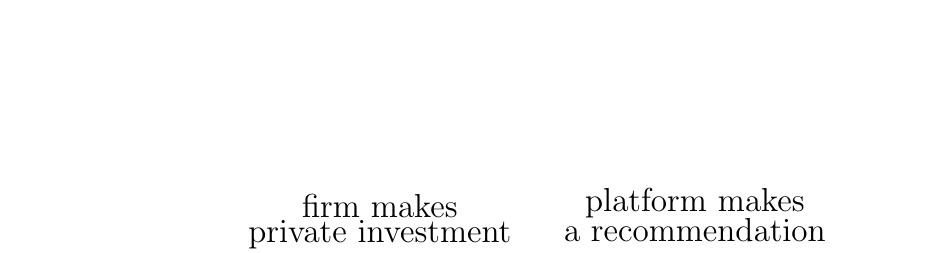
\begin{tikzpicture}
	\draw[ultra thick,->] (0,0) -- (11,0);
	\draw[thick] (1,-0.2) -- (1,0.2);
	\node[label=below:firm learns] at (1,-0.2) {};
	\node[label=below:its state] at (1,-0.5) {};
	\draw[thick] (3,-0.2) -- (3,0.2);
	\node[label=above:firm makes] at (3,0.5) {};
	\node[label=above:private investment] at (3,0.1) {};
	\draw[thick] (5,-0.2) -- (5,0.2);
	\node[label=below:customers] at (5,-0.2) {};
	\node[label=below:arrive] at (5,-0.5) {};
	\draw[thick] (7,-0.2) -- (7,0.2);
	\node[label=above:a recommendation] at (7,0.2) {};
	\node[label=above:platform makes] at (7,0.5) {};
	\draw[thick] (9,-0.2) -- (9,0.2);
	\node[label=below:platform receives] at (9,-0.2) {};
	\node[label=below:reviews] at (9,-0.5) {};
		\end{tikzpicture}
	\caption{Timing}\label{fig1}
	\end{figure}
\end{center}
 	\subsection{Assumptions}
 	Before starting the analysis I would like to explicitly state assumptions the model is based on, and to provide some justifications of these assumptions.
 	\begin{assumption}
 		The platform knows customers' outside options.
 	\end{assumption}
 	This assumption at first glance may seem implausible, however, nowadays platforms have an enormous amount of personal data which can enable them to infer rather precisely about the potential outside option of each customer.
 	
 	\begin{assumption}
 		If the good is not recommended to the customer, then the customer does not consume it. While if the good is recommended the customer may or may not choose it.
 	\end{assumption}
 	This assumption implies that without the platform the customer is unable to find the good. Think about \textit{TripAdvisor}, if it does not show you a restaurant, you will not know about the existence of this restaurant. At the same time, if \textit{TripAdvisor} shows you an option it is up to you whether to go there or not.
 	\begin{assumption}
 		The utility customers obtain in the bad state, $q > 0$ and hence it is always profitable for the platform to recommend the good to at least a small share of customers.
 	\end{assumption}
 This assumption ensures that the platform can get the information about the state of the firm each period.
 \begin{assumption}
 	$p \ge 0.5$
 \end{assumption}
This assumption, on one hand, is pure technical, and simplifies an analysis of optimal policy, but on the other hand it seems reasonable that once the firm invests, the probability that investment will lead to an increase in quality is at least 50\%.
\section{Analysis}
Although the recommender policy the platform employs can be a complicated function of all previous states, I start the analysis from the simplest policy. Namely, I firstly consider the policy that takes into account only the previous realization of the quality of the good.
\subsection{One-round recommendation policy}
Suppose that the platform employs the recommender policy that is based only on the previous period realization of the quality of the good. In this case the policy consists of two shares $\{s^0, s^1\}$ such that $$s_t = \begin{cases}
s^0, \text{ if }\mathcal{Q}_{t-1} = b\\
s^1, \text{ if }\mathcal{Q}_{t-1} = g
\end{cases}$$
The platform should choose $s^0, s^1$ to maximize its objective taking into account incentives of the firm. But firstly as a benchmark consider the first-best case, when the firm always invest. In this case the recommender policy is characterized by the following lemma

\begin{lemma}(First-best)
	If the firm always invests in quality then the optimal recommender policy implies $$s^1_{FB} = s^0_{FB} = p + (1-p)q - \mathcal{P} = \expect[v] - \mathcal{P}$$
\end{lemma}
\begin{proof}
	The proof is straightforward, if the firm invests then the expected quality of the service at each period is $p+(1-p)q$. The platform is maximizing $$\underset{s}{\max}\ (p+(1-p)q - \mathcal{P})s - \frac{s^2}{2}$$ and the solution is given by $$s = p + (1-p)q - \mathcal{P}$$
\end{proof}
Clearly, if the platform implements this policy, the firm does not have incentives to invest in quality. 
\begin{corollary}
	If the firm is strategic then the first-best policy is not implementable i.e. if the platform employs the first-best recommender policy, the firm never invests.
\end{corollary}



The lemma and the corollary above suggest that the optimal policy should induce the firm to invest in quality. The results below give a characterization of the optimal recommender policy.
\begin{lemma}
	Given the recommendation policy $\{s^0, s^1\}$, it is optimal for the firm to invest at the bad state if and only if it is optimal to invest at the good state.
\end{lemma} 
\begin{proof}
	Let $V_{ij}$ be the expected discounted value of the firm which is at state $i$ and in the previous period was at state $j$. Then this values are the solutions to the following system of equations:
	\begin{align}\label{eq1}
	\begin{cases}
	V_{bb} = \mathcal{P}s^0 + \max\{\delta V_{bb}, \delta p V_{gb} + \delta (1-p)V_{bb} - c\}\\
	V_{bg} = \mathcal{P}s^1 + \max\{\delta V_{bb}, \delta p V_{gb} + \delta (1-p)V_{bb} - c\}\\
	V_{gb} = \mathcal{P}s^0 + \max\{\delta V_{bg}, \delta p V_{gg} + \delta (1-p)V_{bg} - c\}\\
	V_{gg} = \mathcal{P}s^1 + \max\{\delta V_{bg}, \delta p V_{gg} + \delta (1-p)V_{bg} - c\}
	\end{cases}
	\end{align}
	In each $\max$ the first component represents the case when the firm does not invest, while the second is the value the firm obtains if invests. 
	
	
	The firm exerts effort at bad state if and only if $$\delta V_{bb} \le \delta p V_{gb} + \delta (1-p)V_{bb} - c \iff V_{gb} - V_{bb} \ge \frac{c}{\delta p}$$
	Similarly, the firm exerts effort at good state if and only if $$V_{gg} - V_{bg} \ge \frac{c}{\delta p}$$ Suppose that the firm exerts effort at bad state, by way of contradiction assume that the firm does not invest at good state. In this case the system of equation becomes
	$$	\begin{cases}
	V_{bb} = \mathcal{P}s^0 + \delta p V_{gb} + \delta (1-p)V_{bb} - c\\
	V_{bg} = \mathcal{P}s^1 + \delta p V_{gb} + \delta (1-p)V_{bb} - c\\
	V_{gb} = \mathcal{P}s^0 + \delta V_{bg}\\
	V_{gg} = \mathcal{P}s^1 + \delta V_{bg}
	\end{cases}$$ and the solution is $$\begin{cases}
	V_{bb} = \frac{1+\delta p - \delta^2p}{(1-\delta)(1+\delta p)}\mathcal{P}s^0 + \frac{\delta^2 p}{(1-\delta)(1+\delta p)}\mathcal{P}s^1 - \frac{c}{(1-\delta)(1+\delta p)}\\
	V_{bg} = \frac{\delta}{(1-\delta)(1+\delta p)}\mathcal{P}s^0 + \frac{1-\delta + \delta p}{(1-\delta)(1+\delta p)}\mathcal{P}s^1 - \frac{c}{(1-\delta)(1+\delta p)}\\
	V_{gb} = \frac{(1+\delta p)(1-\delta)+\delta^2}{(1-\delta)(1+\delta p)}\mathcal{P}s^0 - \frac{\delta^2(1-p)}{(1-\delta)(1+\delta p)}\mathcal{P}s^1 - \frac{c \delta}{(1-\delta)(1+\delta p)}\\
	V_{gg} = \frac{\delta^2}{(1-\delta)(1+\delta p)}\mathcal{P}s^0 + \frac{1 - \delta^2 + \delta p}{(1-\delta)(1+\delta p)}\mathcal{P}s^1 - \frac{c\delta}{(1-\delta)(1+\delta p)}
	\end{cases}$$
	the condition that the firm invest at bad state is
	$$V_{gb} - V_{bb} = \frac{\delta\mathcal{P}}{1+\delta p}(s^1 - s^0) + \frac{c}{1+\delta p} \ge \frac{c}{\delta p}$$
	But this implies
	$$\frac{c}{\delta p} \le \frac{\delta\mathcal{P}}{1 + \delta p}(s^1 - s^0) + \frac{c}{1 + \delta p} = V_{gg} - V_{bg}$$ and hence it is also optimal to invest at good state. The contradiction demonstrates that if the firm invests at the bad state, it also invest at a good state. Using the similar argument it can be shown that investing at the good state also must imply investment at the bad state.
\end{proof}
The result means that either the firm invests at both states or does not invest at all.
The next proposition characterize the policy that induce the firm to invest in quality.
\begin{proposition}\label{prop1}
	Given the recommender policy $\{s^0, s^1\}$, the firm exerts effort at both states if and only if $$s^1 - s^0 \ge \frac{c}{\delta^2 p}$$
\end{proposition}
\begin{proof}
	Suppose the firm does not invest at all, in this case the system \eqref{eq1} becomes
	\begin{align*}
	\begin{cases}
	V_{bb} = \mathcal{P}s^0 + \delta V_{bb}\\
	V_{bg} = \mathcal{P}s^1 + \delta V_{bb}\\
	V_{gb} = \mathcal{P}s^0 + \delta V_{bg}\\
	V_{gg} = \mathcal{P}s^1 + \delta V_{bg}
	\end{cases} \to \begin{cases}
	V_{bb} = \frac{\mathcal{P}s^0}{1-\delta}\\
	V_{bg} = \mathcal{P}s^1 +\frac{\delta}{1-\delta}s^0\\
	V_{gb} = \delta \mathcal{P}s^1 + \frac{1-\delta + \delta^2}{1-\delta}\mathcal{P}s^0\\
	V_{gg} = (1+\delta)\mathcal{P}s^1 + \frac{\delta^2}{1-\delta}\mathcal{P}s^0
	\end{cases}
	\end{align*}
	The necessary condition that ensures that the firm does not invest is $	V_{gb} - V_{bb} < \frac{c}{\delta p}$. Here, $$	V_{gb} - V_{bb} = \delta \mathcal{P}(s^1 - s^0)$$ Hence, the firm will not invest if $s^1 - s^0 < \frac{c}{\delta^2 p \mathcal{P}}$.
	
	
	
	Now suppose, the firm invests in both states. In this case the system \eqref{eq1} becomes
	\begin{align*}
	\begin{cases}
	V_{bb} = \mathcal{P}s^0 + \delta p V_{gb} + \delta(1-p)V_{bb} - c\\
	V_{bg} = \mathcal{P}s^1 + \delta p V_{gb} + \delta(1-p)V_{bb} - c\\
	V_{gb} = \mathcal{P}s^0 + \delta pV_{gg} + \delta(1-p)V_{bg} - c\\
	V_{gg} = \mathcal{P}s^1 + \delta p V_{gg} + \delta (1 - p)V_{bg} - c
	\end{cases}
	\end{align*}
	It is a system of linear equations, and its solution is given by:
	$$\begin{cases}
	V_{bb} = \frac{\delta^2p}{1-\delta}\mathcal{P}s^1 + \frac{1-\delta^2p}{1-\delta}\mathcal{P}s^0 - \frac{c}{1-\delta}\\
	V_{bg} = \frac{1-\delta + \delta^2p}{1-\delta}\mathcal{P}s^1 + \frac{\delta(1-\delta p)}{1-\delta}\mathcal{P}s^0 - \frac{c}{1-\delta}\\
	V_{gb} = \frac{\delta(1-\delta+\delta p)}{1-\delta}\mathcal{P}s^1 + \frac{1-\delta + \delta^2 - \delta^2 p}{1- \delta}\mathcal{P}s^0 - \frac{c}{1-\delta}\\
	V_{gg} = \frac{1 - \delta^2 + \delta^2 p}{1 - \delta}\mathcal{P}s^1 + \frac{\delta^2(1-p)}{1- \delta}\mathcal{P}s^0 - \frac{c}{1 - \delta}
	\end{cases}$$
	and again to ensure that the firm indeed invests one needs to check that $V_{gb} - V_{bb} \ge \frac{c}{\delta p}$. In this case $$V_{gb} - V_{bb} = \delta\mathcal{P}(s^1 - s^0) \ge \frac{c}{\delta p} \iff s^1 - s^0 \ge \frac{c}{\delta^2 p \mathcal{P}}$$
\end{proof}
The result means that the difference in demand of customers that the platform provides the firm with should be high enough to make it optimal for the firm to invest in quality. Also, the straightforward corollary can be obtained
\begin{corollary}
	It becomes harder to encourage firm to invest if either cost of investment $c$ is high, or the probability that investment results in quality increase $p$ is low, or the discount factor $\delta$ is low, ot the priced paid by customers $\mathcal{P}$ is low.
\end{corollary}




The next step is to choose the policy $\{s^0, s^1\}$ to maximize the platform's utility subject to the constraint imposed by the Proposition \ref{prop1}. The following theorem characterize the optimal one-round recommender policy.
\begin{theorem}
	If it is optimal to encourage the firm to invest, then the optimal one-round recommender policy is characterized by $$s^1 = \min \left\{ p + q(1-p) - \mathcal{P} + \frac{c}{\delta^2 p \mathcal{P}} - \frac{c}{\delta \mathcal{P}}, 1\right\}, s^0 = \max\left\{ p + q(1-p) - \mathcal{P} - \frac{c}{\delta \mathcal{P}}, 0\right\}$$
\end{theorem} 
\begin{proof}
	Let $U_i$ be the expected discounted value of the platform if the state of the firm in the previous period was $i$. Then these values are solutions to the following system of equations. 
	\begin{align*}
	&\begin{cases}
	U_b = p\left((1-\mathcal{P})s^0 - \frac{(s^0)^2}{2} + \delta U_g\right) + (1-p)\left((q - \mathcal{P})s^0 - \frac{(s^0)^2}{2} + \delta U_b \right)\\
	U_g = p\left((1- \mathcal{P})s^1 - \frac{(s^1)^2}{2} + \delta U_g\right) + (1-p)\left((q - \mathcal{P})s^1 - \frac{(s^1)^2}{2} + \delta U_b \right)
	\end{cases} 
	\end{align*}
	which can be rewritten as
	\begin{align*}
	\begin{cases}
	U_b = \frac{1}{1 - \delta(1-p)} \left( (p + (1-p)q - \mathcal{P})s^0 - \frac{(s^0)^2}{2} \right) + \frac{p\delta}{1 - \delta(1-p)}U_g\\
	U_g = \frac{1}{1 - \delta p} \left( (p + (1-p)q - \mathcal{P})s^1 - \frac{(s^1)^2}{2} \right) + \frac{(1-p)\delta}{1 - \delta p}U_b
	\end{cases}
	\end{align*}
	the solution is given by
	$$\begin{cases}
	U_b = \frac{1-\delta p}{1-\delta}\left((p + q(1-p) - \mathcal{P})s^0 - \frac{(s^0)^2}{2}\right) + \frac{\delta p}{1-\delta}\left((p + q(1-p) - \mathcal{P})s^1 - \frac{(s^1)^2}{2}\right)\\
	U_g = \frac{\delta (1-p)}{1-\delta}\left((p + q(1-p) - \mathcal{P})s^0 - \frac{(s^0)^2}{2}\right) +\frac{1-\delta(1- p)}{1-\delta}\left((p + q(1-p) - \mathcal{P})s^1 - \frac{(s^1)^2}{2}\right)
	\end{cases}$$
	without loss of generality suppose that at $t = 0$ the firm is at bad state and the platform knows it. Then the platform should solve the following problem
	\begin{align*}
	\underset{s^1, s^0}{\max}&\ \frac{1-\delta p}{1-\delta}\left((p + q(1-p) - \mathcal{P})s^0 - \frac{(s^0)^2}{2}\right) + \frac{\delta p}{1-\delta}\left((p + q(1-p) - \mathcal{P})s^1 - \frac{(s^1)^2}{2}\right)
	\end{align*}
	Clearly $s^1 - s^0 \ge \frac{c}{\delta^2 p \mathcal{P}}$ should bind. Suppose that $s^1 < 1$, we can plug $s^0 = s^1 - \frac{c}{\delta^2 p \mathcal{P}}$ into the objective function. In this case the optimal solution is given by \begin{align}\label{eq2}
	s^0 &= p + q(1-p) - \mathcal{P} - \frac{c}{\delta \mathcal{P}} \nonumber\\
	s^1 &= p + q(1-p) - \mathcal{P} - \frac{c}{\delta \mathcal{P}} + \frac{c}{\delta^2 p \mathcal{P}}
	\end{align}
	We should consider the case $s^1 = 1$, however if $s^1$ obtained in \eqref{eq2} is less than 1, then in case $p \ge 0.5$ it can be shown that the platform's profit is greater for this $s^1$, comparing to $s^1 = 1$.
\end{proof}
As we can see, the optimal one-round recommender policy with the strategic firm differs from the first-best policy when the firm is not strategic. With strategic firm the platform has to "punish" and "reward" the firm by decreasing and increasing the recommended share comparing to the first-best case. Namely, $s^0_{FB} - s^0 = \frac{c}{\delta \mathcal{P}}$, so the amount of punishment decreases once $\delta \to 1$ or $\mathcal{P} \to 1$, and increases once $c \to 1$. Note that if $q > 1 - \frac{c}{\delta p \mathcal{P}} - \frac{\mathcal{P}}{p}$ then $s^0 < q$ which means that the share of customers $q - s^0$ who for sure could derive positive utility from using the good are not recommended doing so. This may suggest that it is not always optimal to induce the firm to invest in quality.



In addition, the recommender policy above is clearly not incentive compatible: those customers whose outside option $r_i \in \left(p+q(1-p) - \mathcal{P}, s^1 \right)$ would rather choose the outside option than follow the recommendation. This is because by following recommendation, given that the firm is investing in quality, the expected utility of the customer is $p + q(1-p) - \mathcal{P}$ while the outside option yields more. But that means that the platform cannot induce the firm to invest in quality since the firm does not obtain enough profit. That is why, the optimal one-round recommender policy with strategic customers should be different from that obtained in this section.


\subsection{Strategic customers}
In this section, I relax the assumption that customers always follow the recommendation, prescribed by the platform. Now, they only do so if and only if the expected utility from choosing the good exceeds the outside option. Formally, 
\begin{definition}
	Given $p, q, \mathcal{P}$, the customer with the outside option $r_i$ would follow the recommendation choosing the good if and only if $$p + (1-p)q - \mathcal{P} \ge r_i$$
\end{definition}

To make some customers willing to follow the recommendation the platform may introduce personal discounts.
\begin{definition}
	The platform employs the personal discount system $d(r_i): [0, 1] \to [0, 1]$ if the price paid by the customer with the outside option $r_i$ is $d(r_i) \cdot \mathcal{P}$
\end{definition}
In other words, by offering a personal discounts the platform makes the good more attractive for  customers. This eventually allows the platform to meet the incentive compatibility constraint of the customers and, as a result, to render the recommender policy incentive compatible.
\begin{theorem}
	If it is optimal to encourage the firm to invest in quality then the best one-round recommender policy embraces recommendations $$s^1 = \min \left\{ p + q(1-p) - \mathcal{P} + \frac{c}{\delta^2 p \mathcal{P}} - \frac{c}{\delta \mathcal{P}}, 1\right\}, s^0 = \max\left\{ p + q(1-p) - \mathcal{P} - \frac{c}{\delta \mathcal{P}}, 0\right\}$$ and the personal discount system $$d(r_i) = \begin{cases}
	1, &r_i \le p + (1-p)q - \mathcal{P}\\
	\frac{p+(1-p)q - r_i}{\mathcal{P}}, &r_i > p + (1-p)q - \mathcal{P}
	\end{cases}$$
\end{theorem}
\begin{proof}
	to be completed
\end{proof}
\section{Extensions}
As for possible extensions, although in the model I consider the simplest class of recommender policies, it would be interesting to consider more general policies ($K$-round policy, $K > 1$). In this case the platform gets more tools to induce the firm to invest, hence, I think the expected social welfare losses from providing the firm with incentives for investing could be lower.




Also, I would be intrigued to see how the optimal policy changes if the firm could charge customers for consuming the good. In this case the firm can use the price as a signal of the quality of the good. 




Finally, it is worth mentioning that the results are based on the assumption that customers are behavioral and always follow the recommendation. I would be interested to see how the policy changes if customers may be strategic. In this case, it would be harder for the platform to induce exploration since it should take into account incentives of customers. 
\section{Conclusion}
Recommender systems became very popular for last years. Several papers have studied the question of optimal design of these systems. While the optimality was mainly understood in terms of inducing exploration of new alternatives for myopic agents. This work is a small step towards another direction. I built a model that was supposed to present a different perspective on the role of the recommender system. Namely, I focused on firm's incentives to maintain the quality of the alternative, and how it can be affected by the policy implemented by the platform. Results demonstrate that the optimal policy should take into account the strategic nature of the firm, and the optimal one-round policy derived in this paper sheds light on how exactly the platform should do it. 


Being very simple, the model I presented can be extended in a variety of directions, that was discussed in the extension section and which I am planing to explore during the future research.


 
\bibliography{lib}{}
\bibliographystyle{unsrt}
\end{document}